\documentclass[12pt]{iopart}
\pdfoutput=1
\usepackage{iopams}
\usepackage{amssymb, epsfig}
%\usepackage{amsmath, amssymb,epsfig}
\usepackage{latexsym}

%\usepackage[hypertex,hyperindex]{hyperref}
%\usepackage{showkeys}
\usepackage{graphicx}
\usepackage{color}

\newcommand{\pf}{\mbox{pf}}
\newcommand{\vep}{\varepsilon}

\begin{document}

\bibliographystyle{plain}
\def\debproof{\noindent {\bf Proof.} }
\def\finproof{\hfill {\small $\Box$} \\}
%\renewcommand{\theequation}{\arabic{section}.\arabic{equation}}
%\tableofcontents
\makeatletter % `@' now normal "letter"
\@addtoreset{equation}{section}
\makeatother  % `@' is restored as "non-letter"
\renewcommand\theequation{{\thesection}.{\arabic{equation}}}

\title[]{Scattering Coefficient and Kirchhoff Approximation}
\author{ }
\address{}



\maketitle

\newcommand{\eps}{\varepsilon}
\newcommand{\RR}{\mathcal{R}}
\newtheorem{lem}{Lemma}[section]
\newtheorem{prop}{Proposition}[section]
\newtheorem{cor}{Corollary}[section]
\newtheorem{thm}{Theorem}[section]
\newtheorem{rem}{Remark}[section]
\newtheorem{alg}{Algorithm}[section]
\newtheorem{assum}{Assumption}[section]
\newtheorem{definition}{Definition}[section]


\newcounter{RomanNumber}
\newcommand{\MyRoman}[1]{\rm\setcounter{RomanNumber}{#1}\Roman{RomanNumber}}

\newcommand{\bL}{\mathbf{L}}
\newcommand{\bH}{\mathbf{H}}
\newcommand{\bW}{\mathbf{W}}
\newcommand{\bP}{\mathbf{P}}
\newcommand{\bQ}{\mathbf{Q}}
\newcommand{\bp}{\mathbf{p}}
\newcommand{\bq}{\mathbf{q}}
\newcommand{\uL}{u_{_{\rm L}}}
\newcommand{\vL}{v_{_{\rm L}}}
\newcommand{\tuL}{\tilde u_{_{\rm L}}}
\newcommand{\tvL}{\tilde v_{_{\rm L}}}
\newcommand{\fL}{f_{_{\rm L}}}
\newcommand{\gL}{g_{_{\rm L}}}
\newcommand{\bpL}{\bp_{_{\rm L}}}
\newcommand{\bqL}{\bq_{_{\rm L}}}
\newcommand{\tbpL}{\tilde{\bp}_{_{\rm L}}}
\newcommand{\tbqL}{\tilde{\bq}_{_{\rm L}}}
\newcommand{\tbpLf}{\tilde{\bp}_{_{\rm L,1}}}
\newcommand{\tbpLs}{\tilde{\bp}_{_{\rm L,2}}}
\newcommand{\tbqLf}{\tilde{\bq}_{_{\rm L,1}}}
\newcommand{\tbqLs}{\tilde{\bq}_{_{\rm L,2}}}
\newcommand{\bn}{\nu}
\newcommand{\bv}{\mathbf{v}}
\newcommand{\om}{\omega}
\newcommand{\pa}{\partial}
\newcommand{\la}{\langle}
\newcommand{\ra}{\rangle}
\newcommand{\lla}{\la{\hskip -2pt}\la}
\newcommand{\rra}{\ra{\hskip -2pt}\ra}
\newcommand{\jj}{\|{\hskip -0.8pt} |}
\newcommand{\al}{\alpha}
\newcommand{\ze}{\zeta}
\newcommand{\si}{\sigma}
\newcommand{\ep}{\varepsilon}
\newcommand{\na}{\nabla}
\newcommand{\vp}{\varphi}
\newcommand{\ga}{\gamma}
\newcommand{\Ga}{\Gamma}
\newcommand{\Om}{\Omega}
\newcommand{\de}{\delta}
\newcommand{\Th}{\Theta}
\newcommand{\De}{\Delta}
\newcommand{\Lam}{\Lambda}
\newcommand{\lam}{\lambda}
\newcommand{\tri}{\triangle}
\newcommand{\lj}{[{\hskip -2pt} [}
\newcommand{\rj}{]{\hskip -2pt} ]}
\newcommand{\bks}{\backslash}
%\newcommand{\diag}{\mathrm{diag}}
\newcommand{\diam}{\mathrm{diam}}
\newcommand{\osc}{\mathrm{osc}}
\newcommand{\meas}{\mathrm{meas}}
\newcommand{\dist}{\mathrm{dist}}

\newcommand{\mL}{\mathscr{L}}
\newcommand{\cT}{{\cal T}}
\newcommand{\cM}{{\cal M}}
\newcommand{\cE}{{\cal E}}
\newcommand{\cL}{{\cal L}}
\newcommand{\cF}{{\cal F}}
\newcommand{\cB}{{\cal B}}
\newcommand{\PML}{{\rm PML}}
\newcommand{\FEM}{{\rm FEM}}
\newcommand{\rd}{\,\mathrm{d}}

\renewcommand{\i}{\mathbf{i}}
\renewcommand{\v}{\mathbf{v}}
\renewcommand{\u}{\mathbf{u}}
\renewcommand{\r}{\mathbf{r}}
\newcommand{\gR}{{\mathbb{R}}}
\newcommand{\Z}{{\mathbb{Z}}}
\newcommand{\C}{{\mathbb{C}}}
\newcommand{\I}{{\mathbb{I}}}
\renewcommand{\Re}{\mathrm{Re}\,}
\renewcommand{\Im}{\mathrm{Im}\,}
\renewcommand{\div}{\mathrm{div}}
\newcommand{\curl}{\mathrm{curl}}
\newcommand{\Curl}{\mathbf{curl}}
\newcommand{\pv}{\mathrm{p.v.}}

\newcommand{\Np}{\mathbb{N}_p}
\newcommand{\Ns}{\mathbb{N}_s}
\newcommand{\Tp}{\mathbb{T}_p}
\newcommand{\Ts}{\mathbb{T}_s}
\newcommand{\Na}{\mathbb{N}_\alpha}
\newcommand{\Nb}{\mathbb{N}_\beta}
\newcommand{\Ta}{\mathbb{T}_\alpha}
\newcommand{\Tb}{\mathbb{T}_\beta}
\newcommand{\GG}{\mathcal{G}}

\newcommand{\N}{\mathbb{N}}
\newcommand{\D}{\mathbb{D}}
\newcommand{\T}{\mathbb{T}}
\newcommand{\A}{\mathbb{A}}
\newcommand{\B}{\mathbb{B}}
\newcommand{\G}{\mathbb{G}}
\newcommand{\F}{\mathbb{F}}
\newcommand{\R}{\mathbb{R}}
\newcommand{\W}{\mathbb{W}}
\newcommand{\V}{\mathbb{V}}
\newcommand{\U}{\mathbb{U}}
\newcommand{\J}{\mathbb{J}}
\newcommand{\Zg}{\mathbb{Z}}
\newcommand{\Gtheta}{\mathbb{\Theta}}
\newcommand{\Gphi}{\mathbb{\Phi}}

%%%%%%%%%%%%%%%%%%%%%%%%%%%%%%%%%%%%%%%%%%%%%%%%%%%%%%%%%%%%%%%%%%%%
\newcommand{\be}{\begin{eqnarray}}
\newcommand{\ee}{\end{eqnarray}}
\newcommand{\ben}{\begin{eqnarray*}}
	\newcommand{\een}{\end{eqnarray*}}
\newcommand{\nn}{\nonumber}

\section{Reflection of Plane Wave}
\subsection{P-wave}
We denote incident P-wave \cite[p172]{achenbach1980} as
\be
u^0=A_0(\sin t_0,\cos t_0)^Te^{\i k_p(x_1\sin t_0+x_2 \cos t_0)}
\ee
and its stress as
\ben
\sigma(u^0)=\i k_p A_0(2\mu \sin t_0\cos t_0,\lambda+2\mu \cos^2 t_0)^Te^{\i k_p(x_1\sin t_0+x_2 \cos t_0)}
\een
The reflected P-wave is represented as
\ben
u^1=A_1(\sin t_1,-\cos t_1)^Te^{\i k_p(x_1\sin t_1-x_2 \cos t_1)}\\
\sigma(u^1)=\i k_p A_1(-2\mu \sin t_1\cos t_1,\lambda+2\mu \cos^2 t_1)^Te^{\i k_p(x_1\sin t_1+x_2 \cos t_1)}
\een
and reflected S-wave as
\ben
u^2=A_2(\cos t_2,\sin t_2)^Te^{\i k_s(x_1\sin t_2-x_2 \cos t_2)}\\
\sigma(u^2)=\i k_sA_2(\mu(\sin^2t_2-\cos^2 t_2),-2\mu\sin t_2\cos t_2)^Te^{\i k_s(x_1\sin t_2-x_2 \cos t_2)}
\een
We consider the clamped condition, then the total field on the $x_2=0$ vanish:
\ben
u^0(x_1,0)+u^1(x_1,0)+u^2(x_1,0)=0
\een
for any $x_1\in \R$. A simple computation show that
\ben
t_1=t_0  \ \ \ \ \ \ \mbox{and} \ \ \ \ \frac{\sin t_2}{\sin t_0}=\frac{k_p}{k_s}:=\kappa \\
A_0=\cos(t_0-t_2) \ \ \ \ \ A_1=\cos(t_0+t_2) \ \ \ \ \ \ A_2=-\sin 2t_0
\een
\subsection{S-wave}
Similarly, we denote incident S-wave as 
\be
u^0=A_0(-\cos t_0,\sin t_0)^Te^{\i k_p(x_1\sin t_0+x_2 \cos t_0)}\\
\sigma(u^0)=\i k_s(\mu(\sin^2t_0-\cos^2 t_0),2\mu\sin t_0\cos t_0)e^{\i k_p(x_1\sin t_0+x_2 \cos t_0)}
\ee
The reflected P-wave is represented as
\ben
u^1=A_1(\sin t_1,-\cos t_1)^Te^{\i k_p(x_1\sin t_1-x_2 \cos t_1)}\\
\sigma(u^1)=\i k_p A_1(-2\mu \sin t_1\cos t_1,\lambda+2\mu \cos^2 t_1)^Te^{\i k_p(x_1\sin t_1+x_2 \cos t_1)}
\een
and reflected S-wave as
\ben
u^2=A_2(\cos t_2,\sin t_2)^Te^{\i k_s(x_1\sin t_2-x_2 \cos t_2)}\\
\sigma(u^2)=\i k_sA_2(\mu(\sin^2t_2-cos^2 t_2),-2\mu\sin t_2\cos t_2)^Te^{\i k_s(x_1\sin t_2-x_2 \cos t_2)}
\een
The result is 
\ben
t_2=t_0  \ \ \ \ \ \ \mbox{and} \ \ \ \ \frac{\sin t_1}{\sin t_0}=\frac{k_s}{k_p}=\frac{1}{\kappa} \\
A_0=\cos(t_0-t_1) \ \ \ \ \ A_1=\sin 2t_0 \ \ \ \ \ \ A_2=\cos(t_0+t_1)
\een

\section{Scattering Coefficient of Elastic Wave}
The solution for the scattering of a plane P-wave  $u_p$(or S-wave $u_s$) with incident direction $d_0$ at a plane $\Gamma := {x \in \R^2 :
	x \cdot \nu = 0}$ through the origin with normal vector $\nu$ is described by
\be
u=u_p + u_{p,p}+u_{p,s}=A_0d_0 e^{\i kp x\cdot d}+A_1 d_1 e^{\i kp x\cdot d_1}+A _2d_2^\perp d_0^{\i ks x\cdot d_2}\\
u=u_s + u_{s,p}+u_{s,s}=A_0d_0^\perp e^{\i ks x\cdot d}+A_1 d_1 e^{\i kp x\cdot d_1}+A_2 d_2^\perp d^{\i ks x\cdot d_2}
\ee
where $d_i=(d_i^1,d_i^2)^T$ are unit vectors, $d_i^\perp=(d_i^2,-d_i^1)^T$ and $A_i$ are corresponding amplitude. For fixed boundary, we have $u=0$ for $x\in\Gamma$. After a standard computation, we get
for P-wave:
\be
d_1= d_0- 2\alpha\nu\\
d_2= \kappa d_0- \beta\nu\\
A_0=\kappa(d,\nu)^2-\kappa(d,\nu^\perp)^2-\beta(d,\nu)\\
A_1=\kappa-\beta(d,\nu)\\
A_2=-2(d,\nu)(d,\nu^\perp)
\ee
where $\alpha=(d,\nu)$, $\beta=\kappa\alpha-\sqrt{\kappa^2\alpha^2-\kappa^2+1}$ and $\kappa=k_p/k_s$. For S-wave:
\be
d_1 =\kappa_1 d_0- \gamma\nu \\
d_2 =d_0- 2\alpha\nu\\
A_0=\kappa_1(d,\nu)^2-\kappa_1(d,\nu^\perp)^2-\gamma(d,\nu)\\
A_1=2(d,\nu)(d,\nu^\perp)\\
A_2=\kappa_1-\gamma(d,\nu)
\ee
where $\gamma=\kappa_1\alpha-\sqrt{\kappa_1^2\alpha^2-\kappa_1^2+1}$ and $\kappa_1=1/\kappa$. Thus the traction of $u(x)$ on the plane $\Gamma$ can be obtained. For P-wave
\ben
\sigma(u)\cdot\nu=[\i k_p A_0 (\lambda\nu+2\mu(d_0,\nu)d_0)+\i k_p A_1 (\lambda\nu+2\mu(d_1,\nu)d_1)\\+\i k_s A_2\mu((d_2,\nu)d_2^\perp+(d_2^\perp,\nu)d_2)]e^{\i k_p x\cdot d}:=\i k_p \hat R_p(x,d,\nu) e^{\i k_p x\cdot d}
\een For S-wave
\ben
\sigma(u)\cdot\nu=[\i k_s A_0 \mu((d_0,\nu)d_0^\perp+(d_0^\perp,\nu)d_0)+\i k_p A_1 (\lambda\nu+2\mu(d_1,\nu)d_1)\\+\i k_s A_2\mu((d_2,\nu)d_2^\perp+(d_2^\perp,\nu)d_2)]e^{\i k_s x\cdot d}:=\i k_s \hat R_s(x,d,\nu) e^{\i k_s x\cdot d}
\een
\begin{definition}
	For any unit vector $d\in \R^2$, let $u^i_p =d e^{\i k_p x\cdot d}$ or $u^i_s= d^\perp e^{\i k_s x\cdot d}$ be the incident wave and $u^s_\alpha = u^s_\alpha(x;d)$ be the radiation solution of the Navier equation:
	\be
	u^s_\alpha + \om^2u^s_\alpha = 0\ \ \mbox{in} \ \  \R^2\bks\bar{D} \\
	u^s_\alpha =-u^i_\alpha \ \ \mbox{on} \ \ \pa D 
	\ee
	The scattering coecient R(x;d) for $x\in\pa D$ is defined by the relation
	\ben
	\sigma(u^s_\alpha+u^i_\alpha)\cdot \nu= \i k_\alpha R_\alpha(x;d)e^{\i k_\alpha x\cdot d}  \ \ \ \mbox{on}\ \ \pa D
	\een
	where $\alpha=p,s$.
\end{definition}
A convex object $D$ locally may be cosidered at each point $x$ as a plane with normal $\nu(x)$. Then the scattering coefficient can be approximated by
\ben
R_\alpha(x;d)\approx\left\{ \begin{array}{ll}
	\hat R_\alpha(x;d,\nu)    \ \  \  \mbox{if} \ \ x \in \pa D^{-}_d=\{x\in \pa D, \nu(x)\cdot d<0\},\\ 
	0 \ \ \ \ \ \ \ \  \ \ \ \ \ \ \ \ \ \mbox{if} \ \ x \in \pa D^{-}_d=\{x\in \pa D, \nu(x)\cdot d\geq0\}.
\end{array} \right.
\een
\begin{figure}
	\centering
	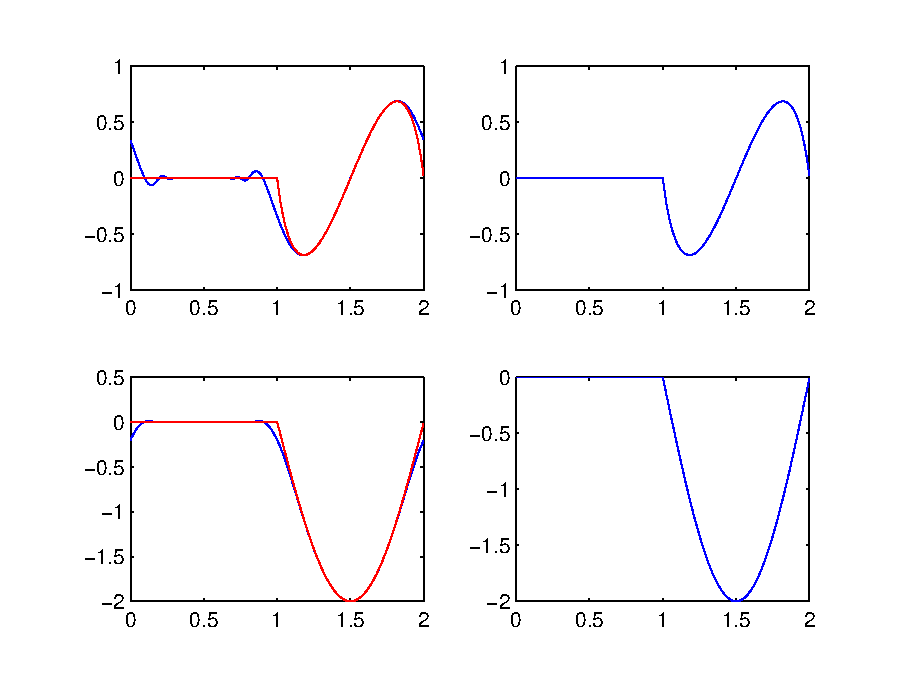
\includegraphics[width=0.8\textwidth]{./graphic/pwave_kirchhoffpi0.eps}
	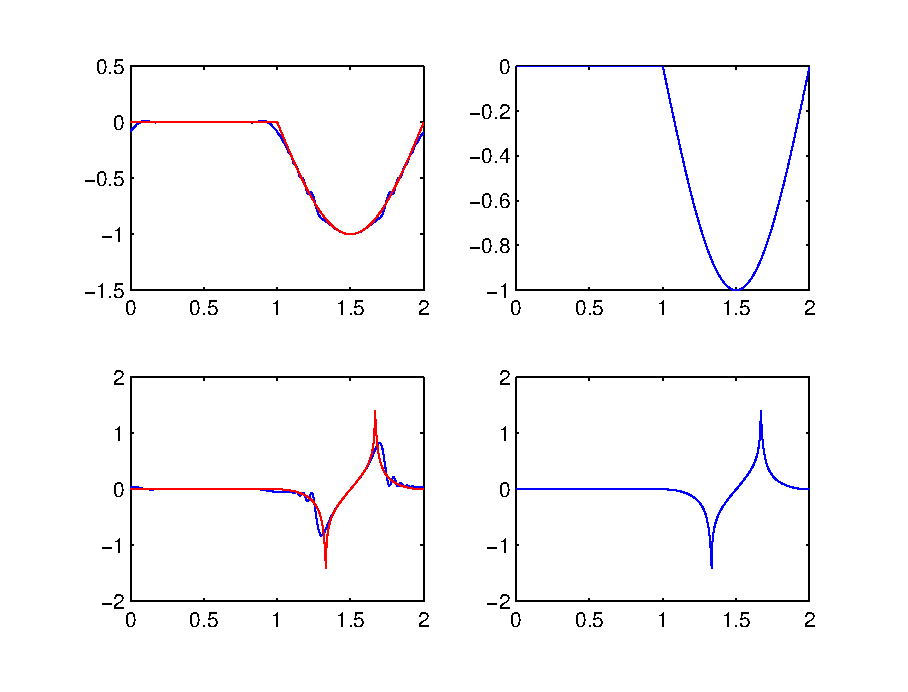
\includegraphics[width=0.8\textwidth]{./graphic/swave_kirchhoffpi0.eps}	
	\caption{$\theta=0\pi$}\label{figure_1}
\end{figure}
\begin{figure}
	\centering
	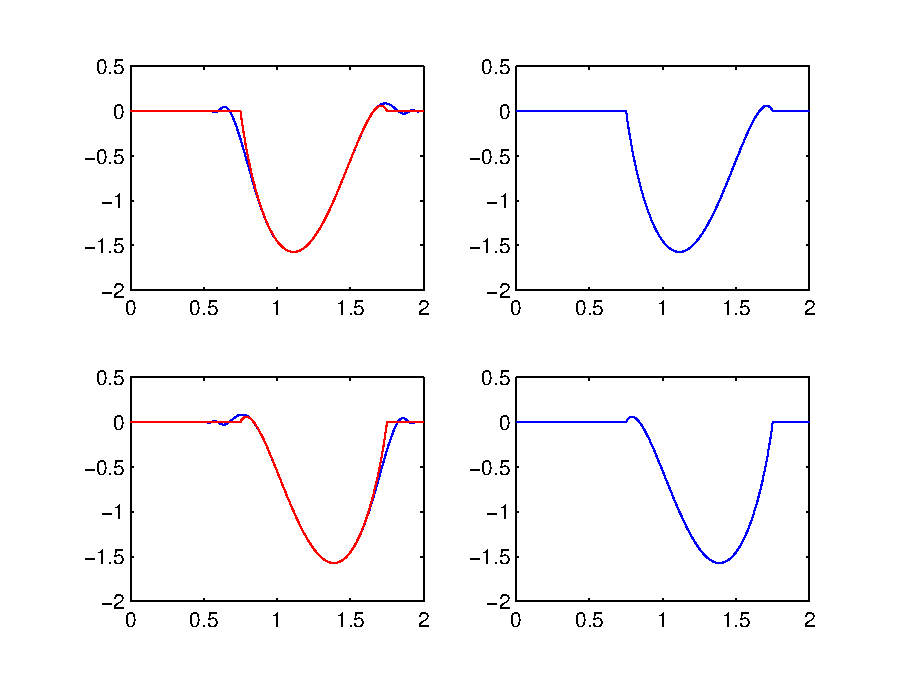
\includegraphics[width=0.8\textwidth]{./graphic/pwave_kirchhoff.eps}
	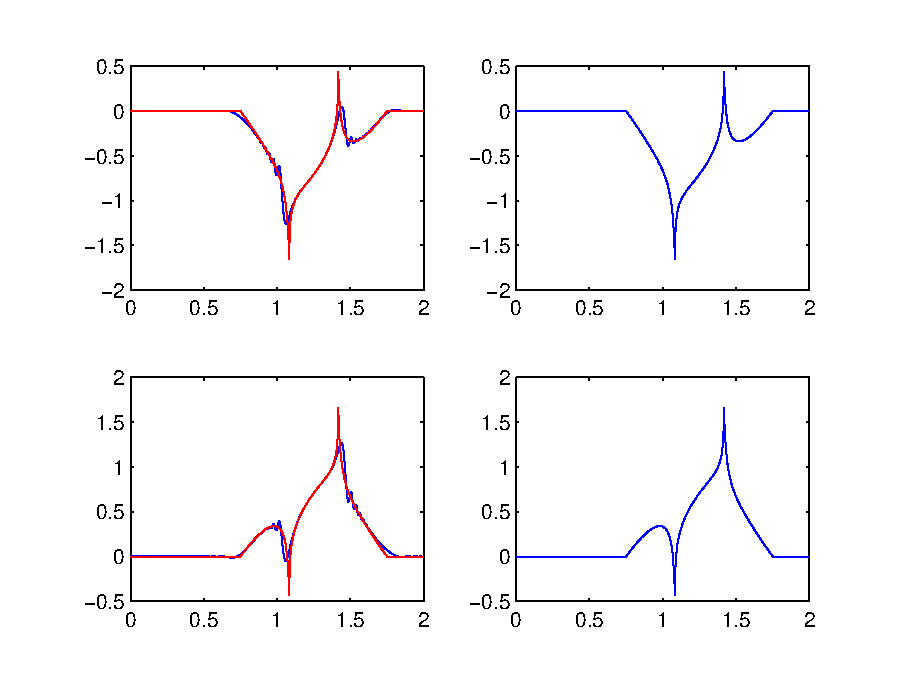
\includegraphics[width=0.8\textwidth]{./graphic/swave_kirchhoff.eps}	
	\caption{$\theta=pi/4$}\label{figure_2}
\end{figure}
\begin{figure}
	\centering
	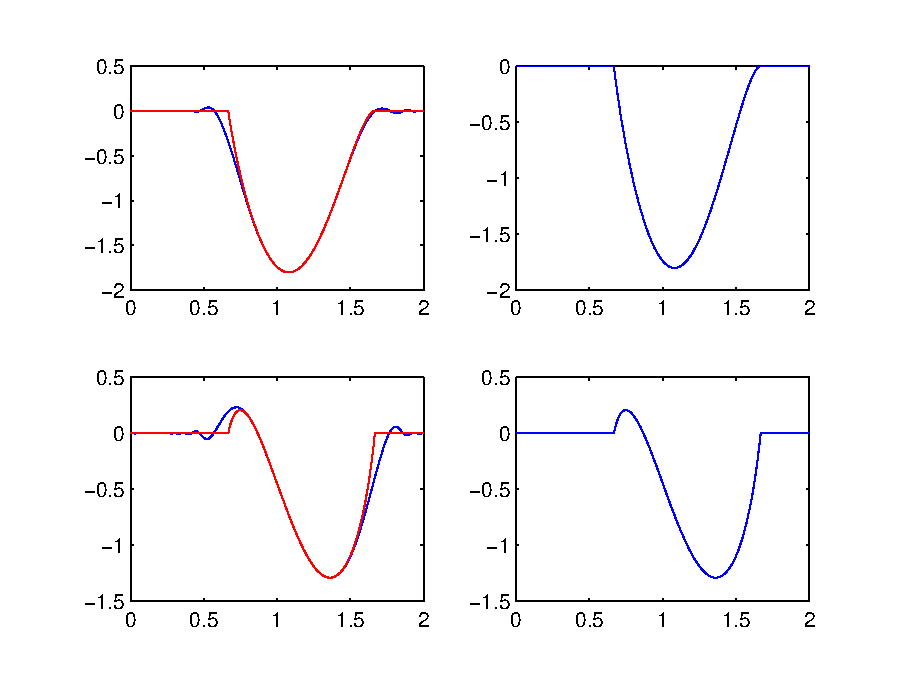
\includegraphics[width=0.8\textwidth]{./graphic/pwave_kirchhoffpi3.eps}
	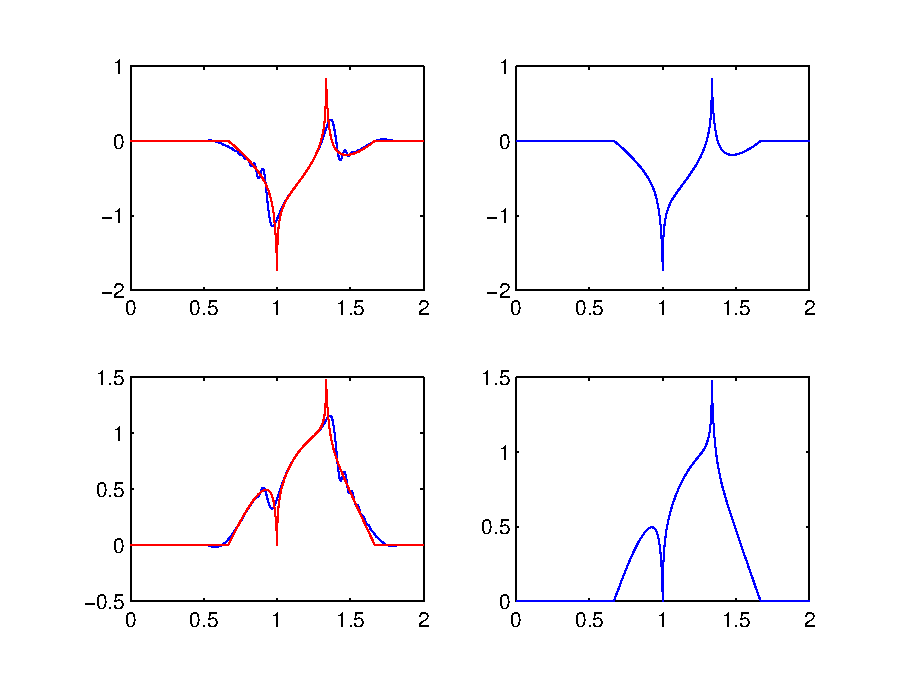
\includegraphics[width=0.8\textwidth]{./graphic/swave_kirchhoffpi3.eps}	
	\caption{$\theta=\pi/3$}\label{figure_3}
\end{figure}
\section*{References}
\begin{thebibliography}{99}
	\bibitem{achenbach1980}
	Achenbach J 1980 {\em Wave Propagation in Elastic Solids }(North-Holland)
	
\end{thebibliography}
\end{document}
